\فصل{تصویرسازی سامانه‌ها}
در فصل‌های گذشته تنها با ثبت عددی خروجی‌های مدلسازی سروکار داشتیم. خروجی‌ها تلاش داشتند تا رفتار سامانه را به ما بشناسانند. ما نیز تلاش کردیم تا بررسی اشکال و نمودارها آنچه را که در پس‌پرده [جعبه سیاه] می‌گذرد؛ «حدس» بزنیم. به همین دلیل برآن شدیم تا روشی برای به تصویر کشیدن سامانه ابداع کنیم تا از لحظه‌لحظه‌ی سامانه با خبر شویم. شکل \ref{fig:if_animation_plot}

\begin{figure}[!h]
	\centering
	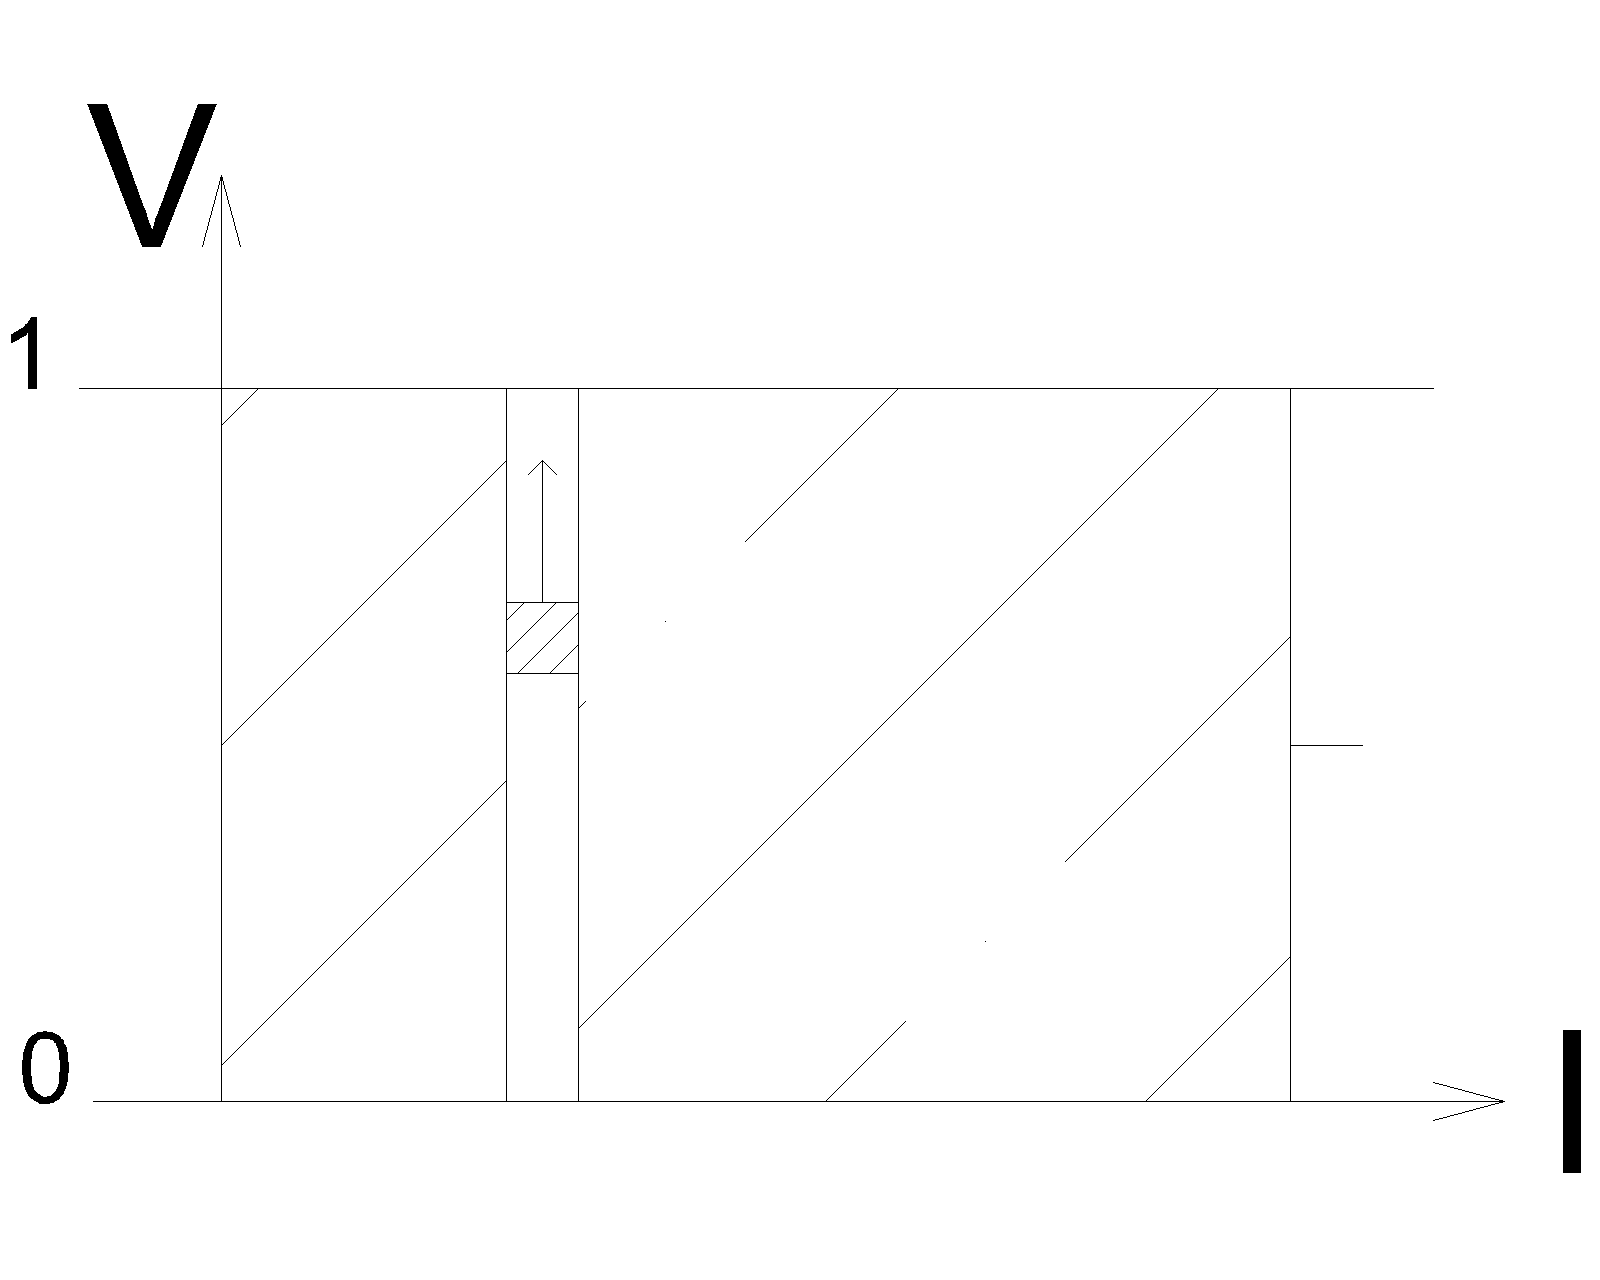
\includegraphics[width =0.8\textwidth]{../papers_studies/figs/IF/IF_phase_space-Model.png}
	\caption{تصویر فضای فاز سامانه نورونی انباشت‌وشلیک}
	\label{fig:if_animation_plot}
\end{figure}

هر نقطه در این صفحه نمایانگر حالت یک نورون است. محور افقی نشان دهنده‌ی جریان ثابت خارجی است که به هر نورون در ابتدا متصل کرده‌ایم و محور عمودی نشان دهنده‌ی پتانسیل نورون است. پویایی شکل \ref{fig:if_animation_plot} به ما نشان خواهد داد که چگونه سامانه در زمان متحول می‌شود. طبق توصیفی که از پویایی سامانه‌ی خود داریم؛ توقع داریم که نورون‌هایی که از آستانه عبور کردند؛ مجددا از محور صفر پیدا شوند.\\

حال بیایید تا پویایی مدل‌های مختلف سامانه‌های نورونی را از این طریق رصد کنیم. به این ترتیب که برای هر کدام از نقاطی خاص از فضای فاز مربوط به آن‌ها انتخاب می‌کنیم و می‌پرسیم که سامانه چه تصویری دارد.\\
در شکل‌ 
\ref{fig:abc_points_neuron_models}
از هر صفحه‌ی فاز ۴ نقطه به اختصار انتخاب شده است.
\begin{enumerate}[a.]
	\item 
	نقطه‌ی 
	A
	:معرف نقطه‌ای است که سامانه دقیقا در حالت هم‌گام قرار دارد.
	\item 
	نقطه‌ی
	B
	:نقطه‌ای میانی بین فاز هم‌گام و ناهم‌گام است.
	\item 
	نقطه‌ی
	C
	: حالتی ناهم‌گام است با این وجود که تاخیر آکسونی در سامانه وجود دارد اما هم‌گامی رخ نمی‌دهد.
	\item 
	D
	: حالتی از سامانه است که ضریب تاثیر قابل ملاحظه‌ای دارد اما تاخیر در سامانه نزدیک به صفر است.
\end{enumerate}
برای مشاهده‌ی کامل پویانمایی‌هاپوشه‌ی مربوط به هر مدل مراجعه کنید:
\href{run://..//scripts//all_neurons_model_in_one_place//animations//sea_shore//black_white}{پوشه‌ی پویانمایی}

\begin{figure}[!h]
	\begin{subfigure}{0.5\textwidth}
	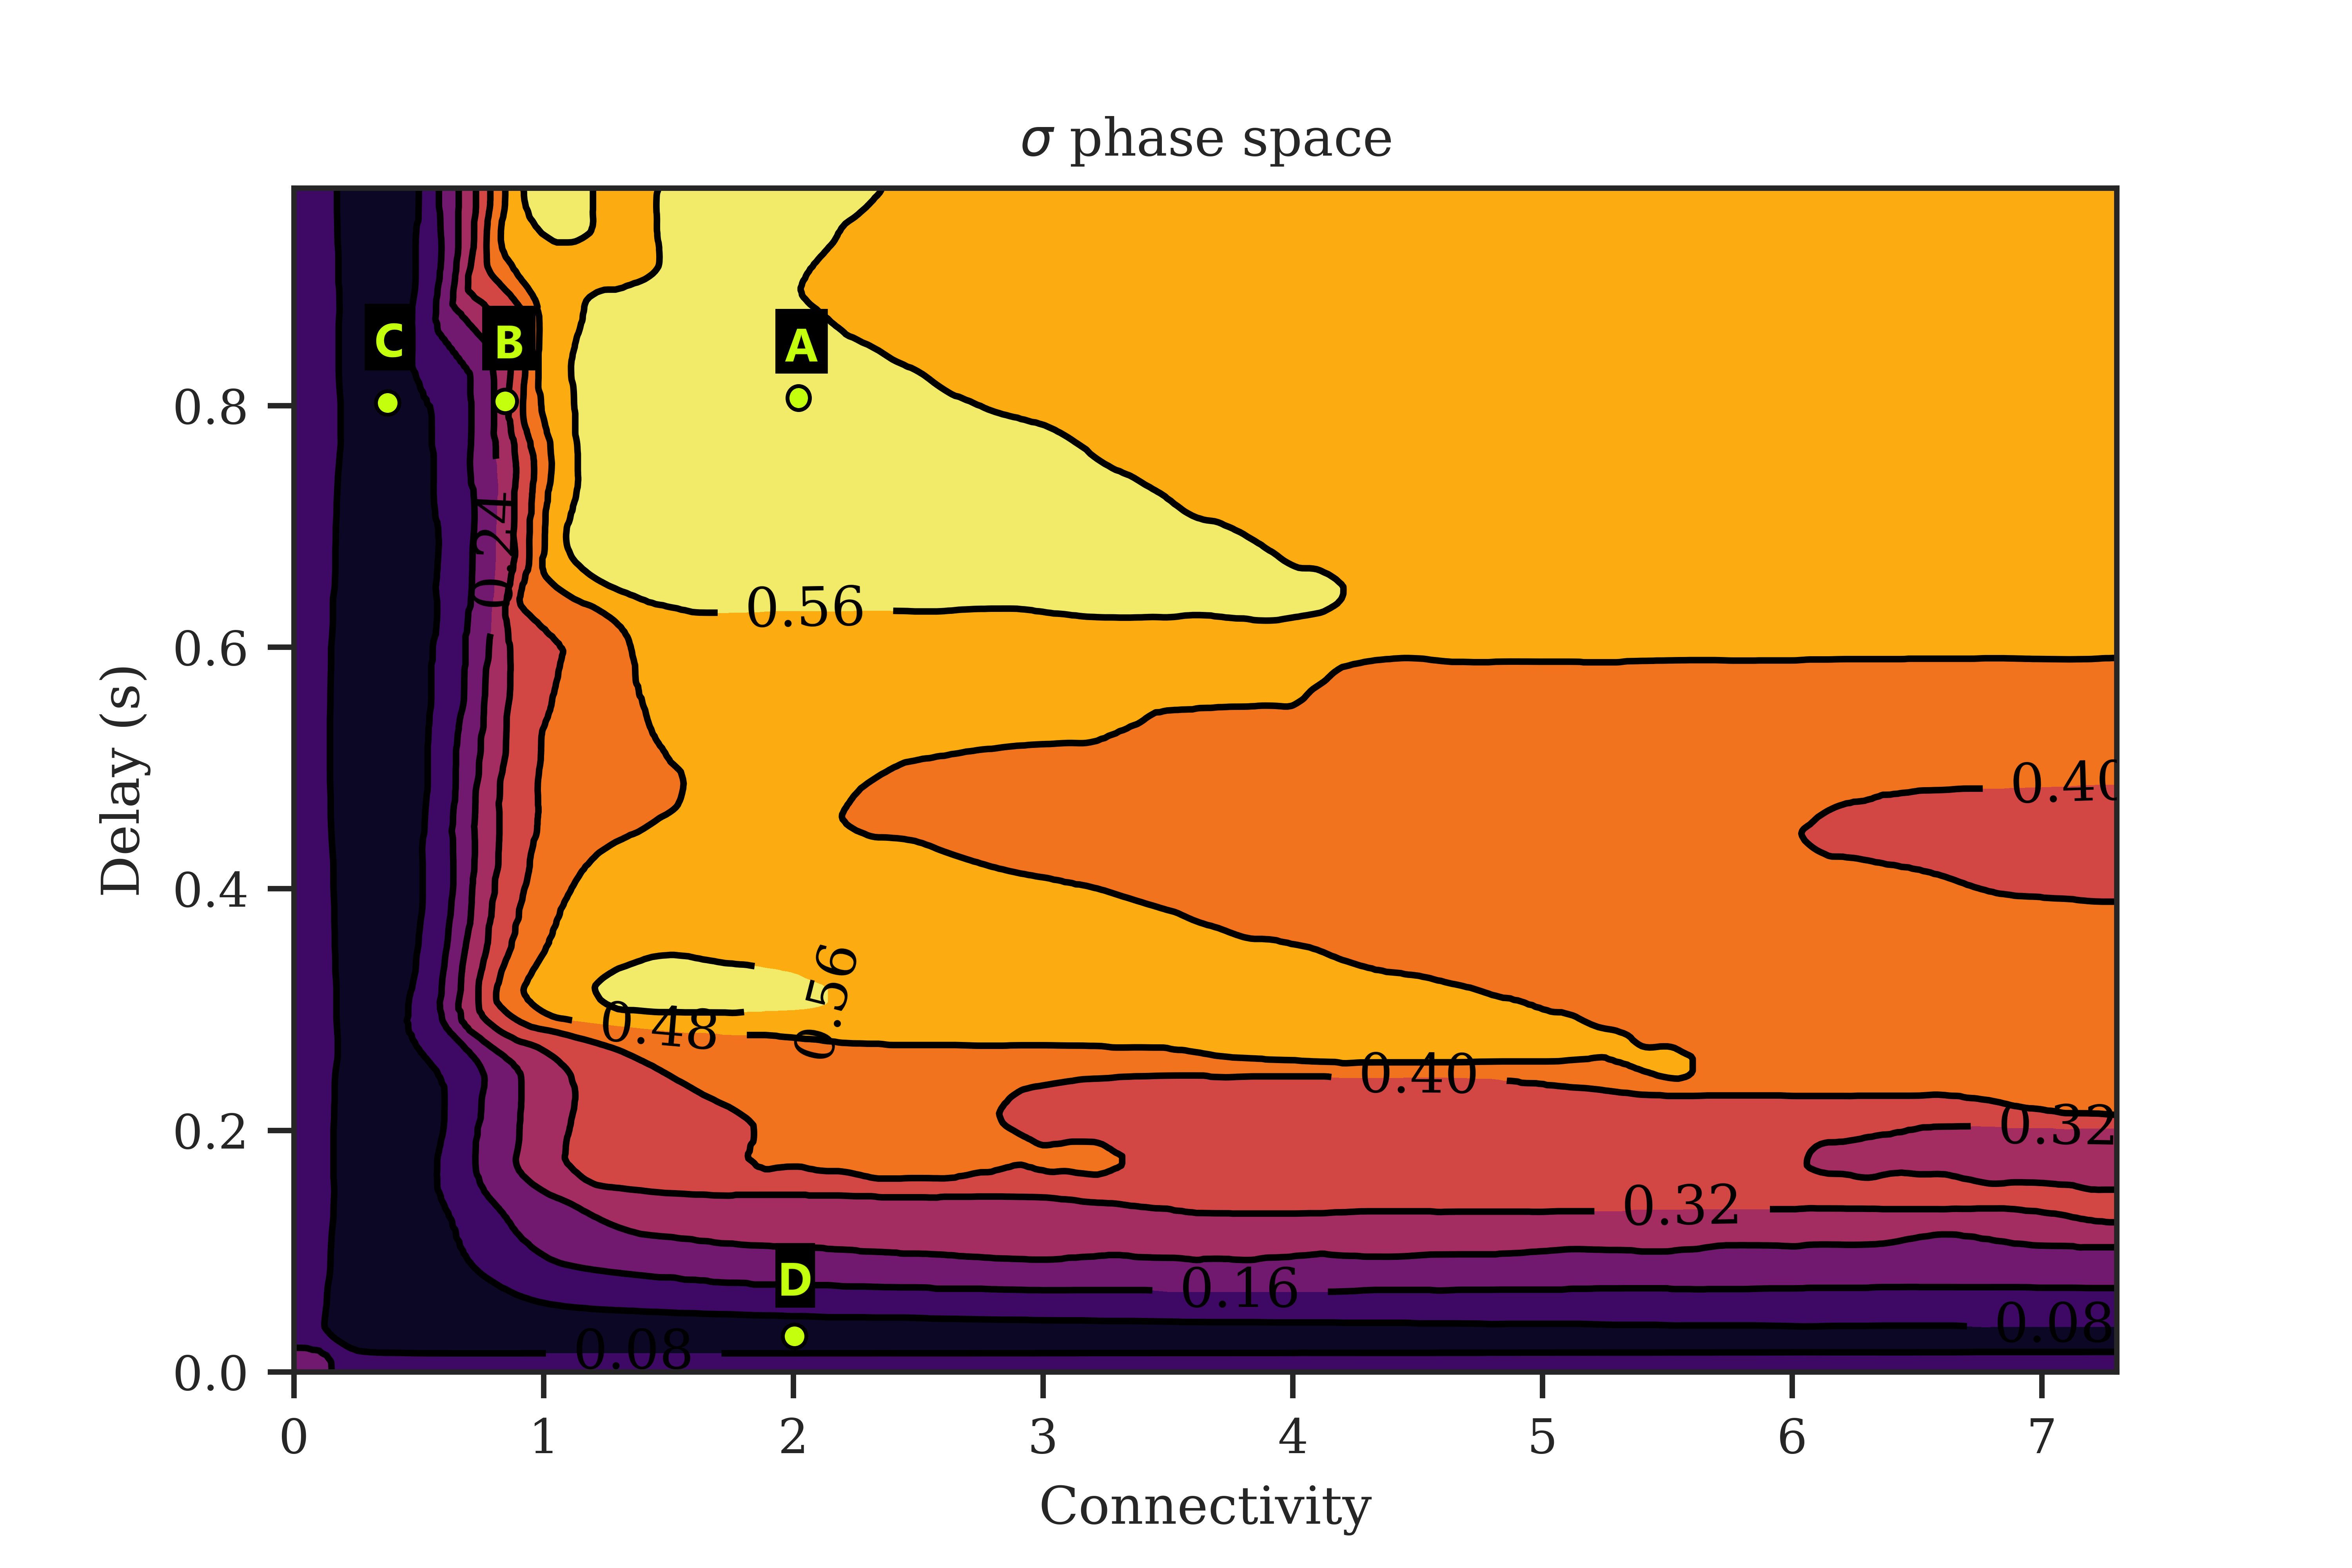
\includegraphics[width = \textwidth]{Figures/animation_chapter/IF_sigma_phase_space_contour_selected_points.png}
	\caption{
		نقاط انتخاب شده در فضای فاز شبکه‌ی نورون‌های انباشت‌وشلیک
	}
	\label{fig:IF_abc}
	\end{subfigure}
	\hfill
	\begin{subfigure}{0.5\textwidth}
		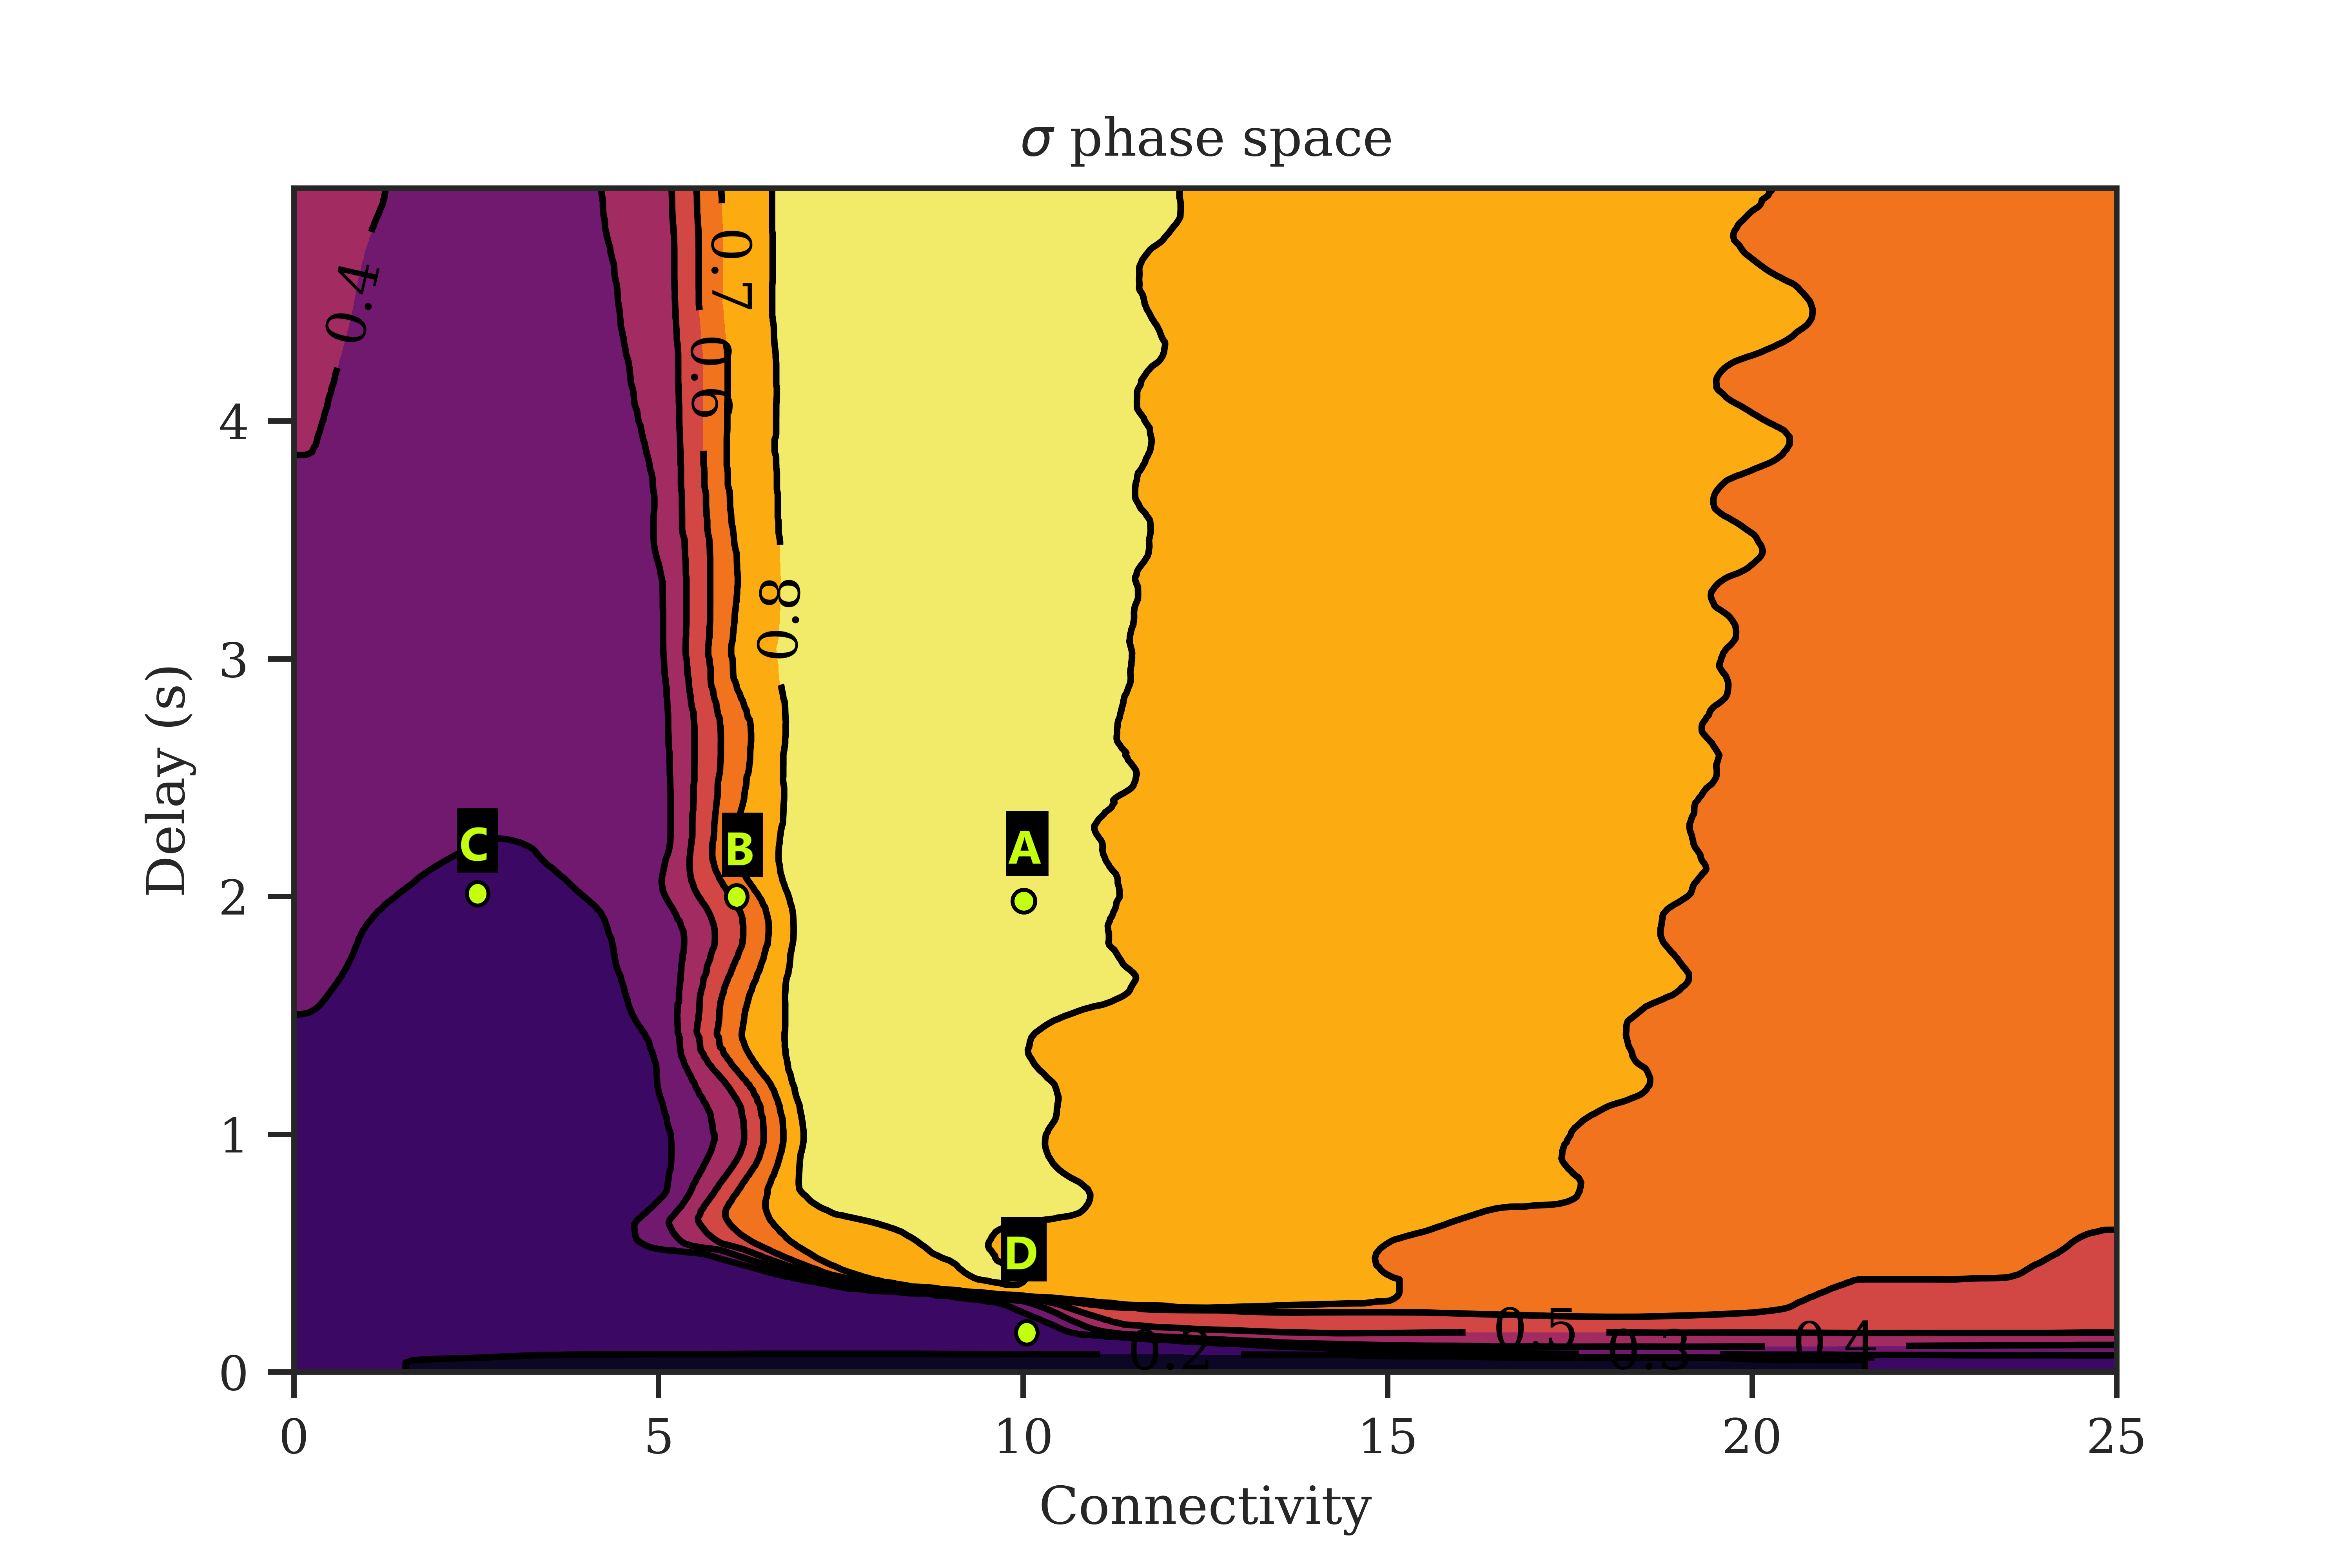
\includegraphics[width = \textwidth]{Figures/animation_chapter/Rotational_sigma_phase_space_contour_selected_points.png}
		\caption{
		نقاط انتخاب شده در فضای فاز شبکه‌ی نورون‌های چرخنده
	}
		\label{fig:Rotational_abc}
	\end{subfigure}
	\hfill
	\begin{subfigure}{0.5\textwidth}
		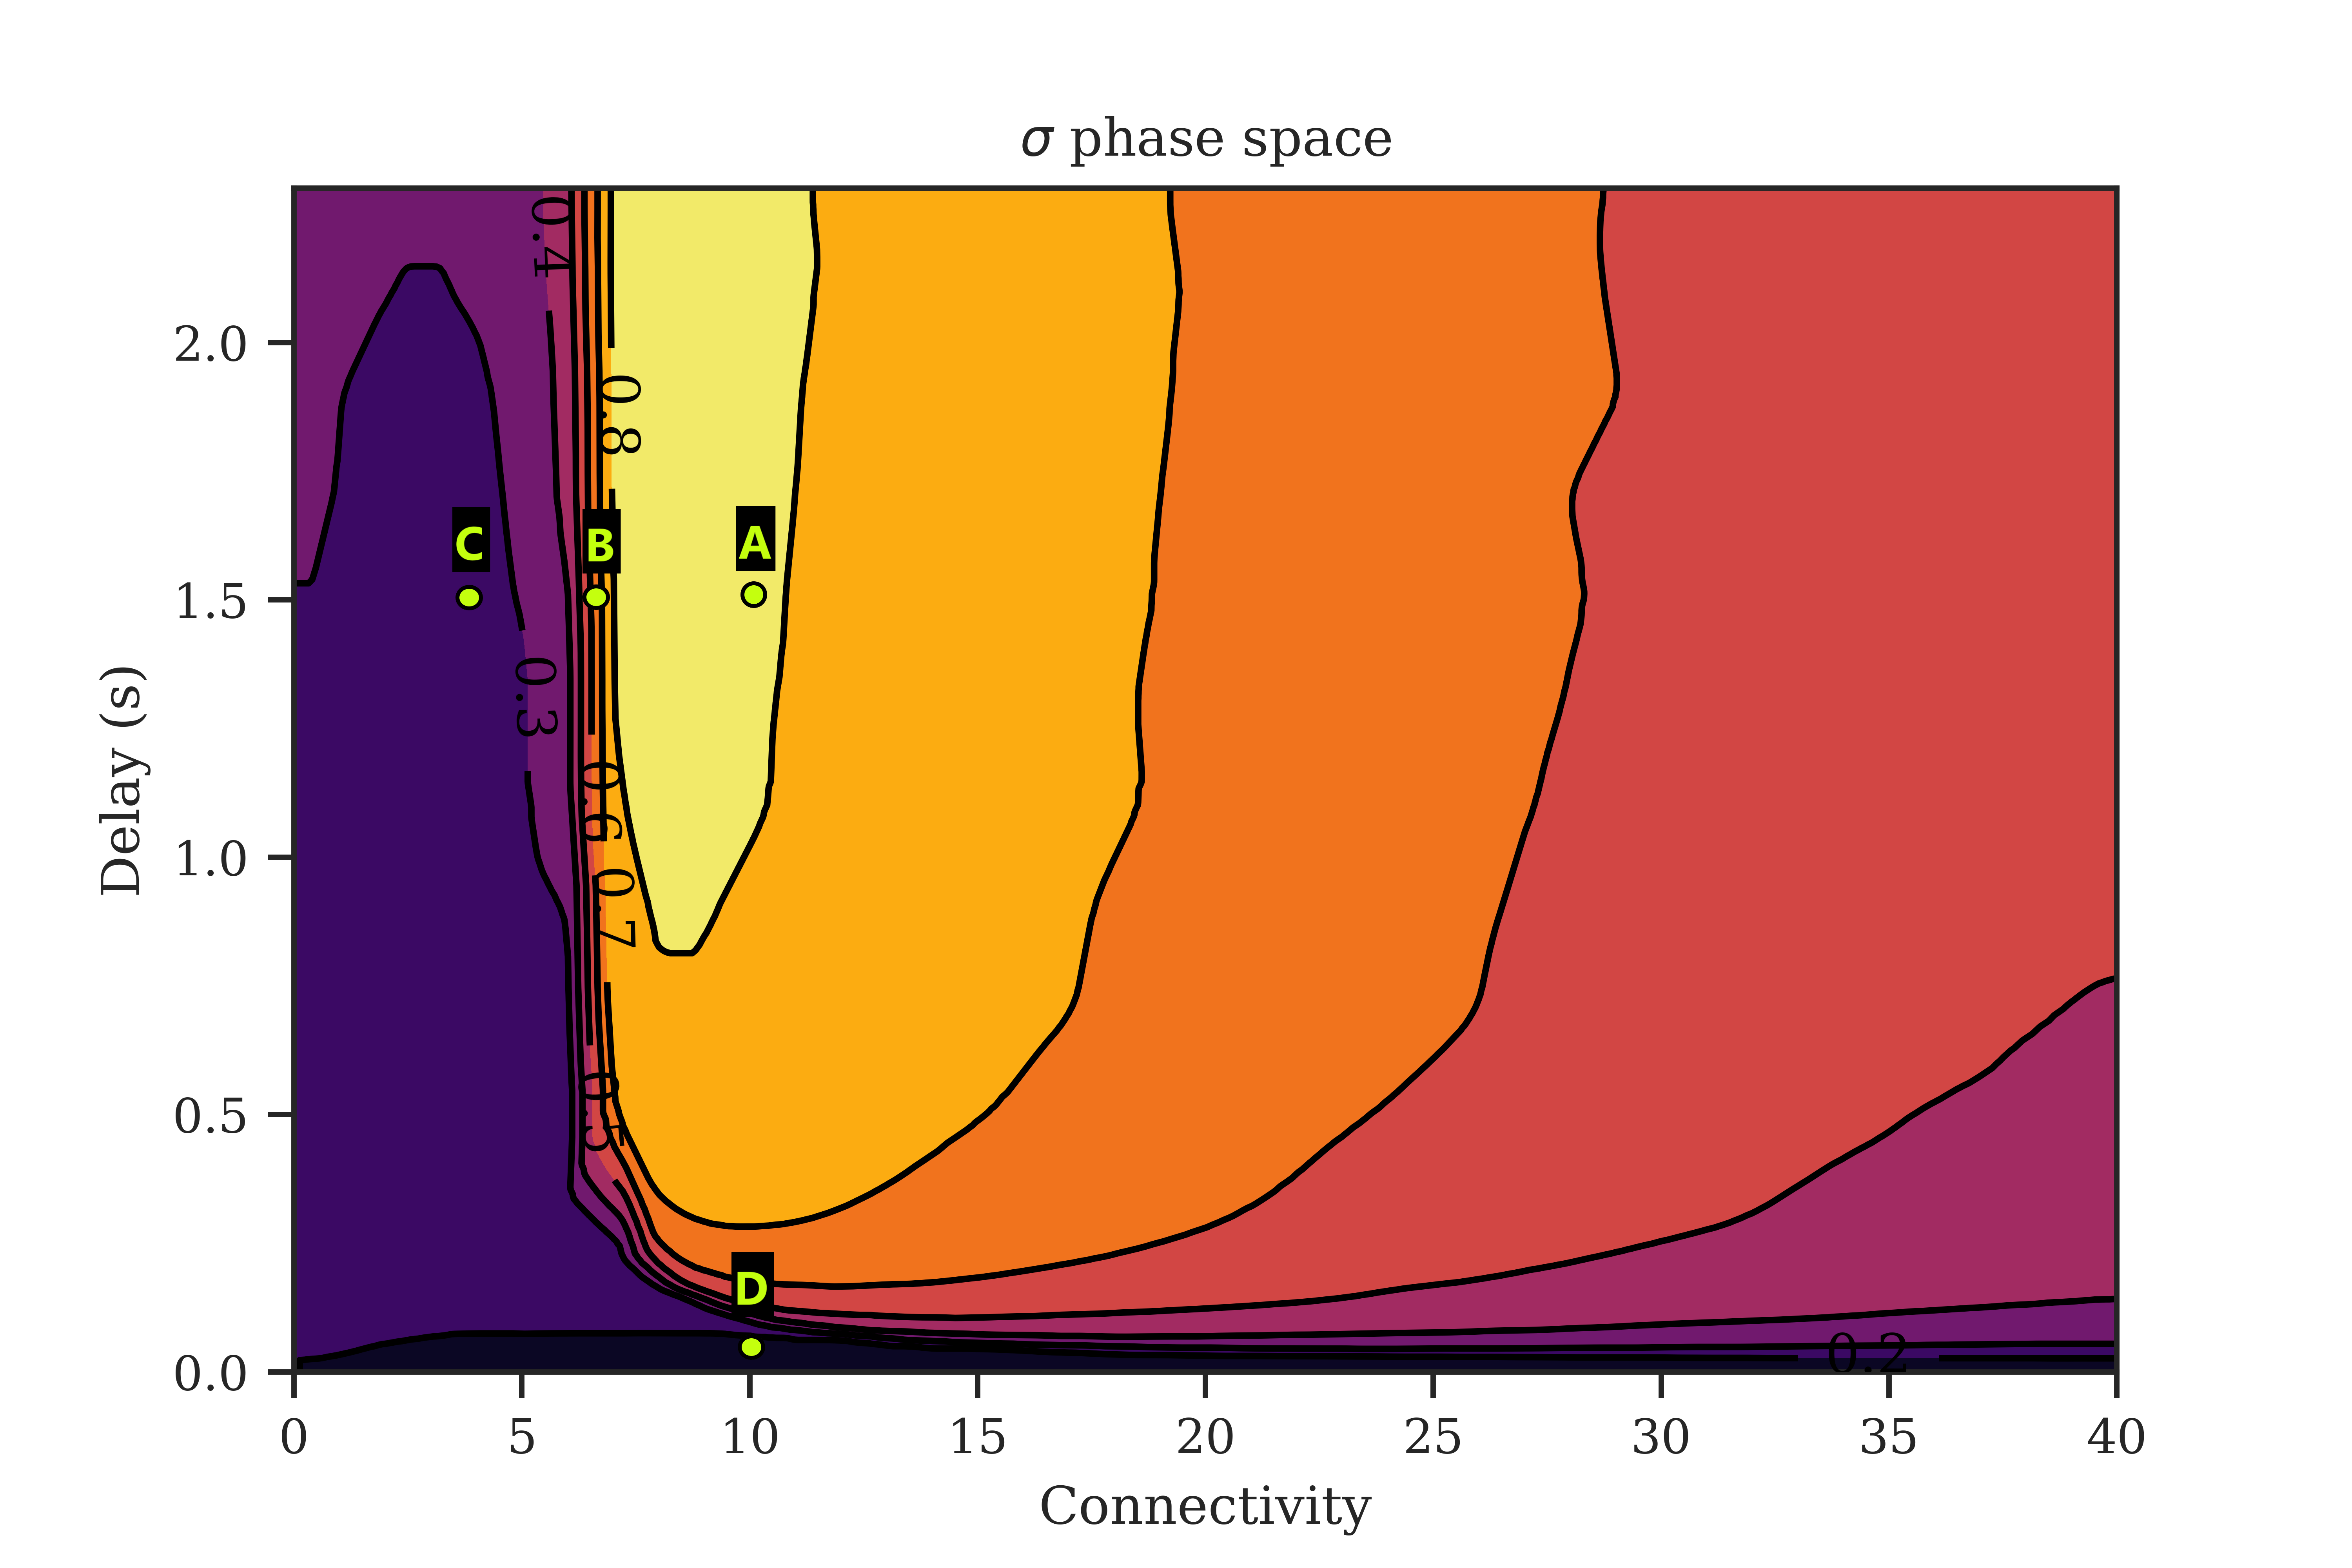
\includegraphics[width = \textwidth]{Figures/animation_chapter/Non_repulsive_sigma_phase_space_contour_alpha20_selected_points.png}
		\caption{
		نقاط انتخاب شده در فضای فاز شبکه‌ی نورون‌های ساده
		}
		\label{fig:Non_repulsive_abc}
	\end{subfigure}
	\hfill
	\caption{}
	\label{fig:abc_points_neuron_models}
\end{figure}

\newpage
\قسمت{پویانمایی}
\زیرقسمت{مدل انباشت‌وشلیک}
شکل
\ref{fig:IF_animation_A}
نمایی از ۶ برداشت از پویانمایی سامانه‌ی نورون‌های انباشت‌وشلیک ارائه شده است. شرایط اولیه این سامانه به گونه‌ای است که همه‌ی نورون‌ها در فضای فاز به صورت یکنواخت توزیع شده‌اند. تو گویی حالت اولیه شبکه یک مستطیل یکنواخت را روایت می‌کرده است.\\
بیاید ورقی بزنیم و به نکاتی این زنجیره از اشکال با خود دارد بپردازیم:
\begin{description}
	\item[تجمع فازها] 
	نمای سامانه در این حالت بسیار قابل توجه است. همه‌ی نورون‌هایی که جریان خارجی مشخصی دارند؛ در یک فاز جمع شده‌اند.
	\item[نورون‌های همسایه] 
	 فاصله‌ی فاز هر دو نورون با جریان خارجی نزدیک به هم رابطه‌ای خطی دارد. این پیشامد نیز با بازنویسی معادلات دیفرانسیل قابل درک است.
	 \begin{align}
	 	\dot{v_a} &= a - v_a - g E\\
	 	\Delta\dot{v_a} &= \Delta a - \Delta v_a\\
	 	\frac{\Delta\dot{v_a}}{\Delta a} &= 1 - \frac{\Delta v_a}{\Delta a}\\
	 	\Rightarrow \frac{\Delta v_a}{\Delta a} &= 1 + C_0 e^{-t}\\
	 	\Rightarrow \frac{\Delta v_a}{\Delta a} &\rightarrow 1
	 \end{align}
 پس این معادلات کاملا توضیح می‌دهد که فارغ از شرط اولیه در صفحه‌ی فاز باید انتظار یک خط با شیب یک داشته باشیم که همه‌ی نورون‌ها در آن جمع شده‌اند. در کنار این شرط دوره‌ای هم باید در نظر گرفته شود که باعث شده است این خط بریده‌بریده شود.
 	\item[جفت شدن سرعت‌ها]
 	هم‌گامی در این شکل به معنای جفت شدن سرعت‌های نورون‌ها با یکدیگر است و نه فاز آن‌ها. آن‌ها با هم به سمت آستانه حرکت می‌کنند و باهم عقب‌نشینی می‌کنند اما دوشادوش یک‌دیگر کمتر قرار می‌گیرند.\\
 	بیاید به معادلات قسمت قبل دوباره نگاه کنیم. می‌توانیم نتیجه بگیریم تفاوت سرعت‌های دو نورون با جریان‌های پشت سرهم صفر خواهد بود.
 	\begin{align}
 		\Delta\dot{v_a} &= \Delta a - \Delta v_a\\
 		&= \Delta a (1 - \frac{\Delta v_a}{\Delta a}) \rightarrow 0
 	\end{align}
 	به این ترتیب می‌توان فهمید این فازها نیستند که باهم جفت می‌شوند 
 	($\Delta v_a \nrightarrow 0 $)
 	بلکه این سرعت‌ها هستند که بهم قفل می‌شوند
 	($\Delta \dot{v_a} \rightarrow 0 $)
\end{description}

\newpage
\begin{figure}[!h]
	\begin{subfigure}{0.5\textwidth}
		\includegraphics[width = \textwidth]{../scripts/all_neurons_model_in_one_place/animations/sea_shore/black_white/IF_frames/A/1.png}
		\caption{
			ثانیه صفرم		
		}
		%		\label{}
	\end{subfigure}
	\hfill
	\begin{subfigure}{0.5\textwidth}
		\includegraphics[width = \textwidth]{../scripts/all_neurons_model_in_one_place/animations/sea_shore/black_white/IF_frames/A/50.png}
		\caption{
			ثانیه $0.5$
		}
		%		\label{}
	\end{subfigure}
	\hfill
	\begin{subfigure}{0.5\textwidth}
		\includegraphics[width = \textwidth]{../scripts/all_neurons_model_in_one_place/animations/sea_shore/black_white/IF_frames/A/100.png}
		\caption{
			ثانیه $1$		
		}
		%		\label{}
	\end{subfigure}
	\hfill
	\begin{subfigure}{0.5\textwidth}
		\includegraphics[width = \textwidth]{../scripts/all_neurons_model_in_one_place/animations/sea_shore/black_white/IF_frames/A/150.png}
		\caption{
			ثانیه $1.5$
		}
		%		\label{}
	\end{subfigure}
	\hfill
	\begin{subfigure}{0.5\textwidth}
		\includegraphics[width = \textwidth]{../scripts/all_neurons_model_in_one_place/animations/sea_shore/black_white/IF_frames/A/200.png}
		\caption{
			ثانیه $2$
		}
		%		\label{}
	\end{subfigure}
	\hfill
	\begin{subfigure}{0.5\textwidth}
		\includegraphics[width = \textwidth]{../scripts/all_neurons_model_in_one_place/animations/sea_shore/black_white/IF_frames/A/250.png}
		\caption{
			ثانیه $2.5$
		}
		%		\label{}
	\end{subfigure}
	\hfill
	\caption{
		نمایی از پویایی سامانه‌ی نورونی انباشت‌وشلیک در نقطه‌ی A - این پویانمایی پس گذشت ۲۰۰ ثانیه از تاریخچه‌ی سامانه انجام شده است. شرایط اولیه به گونه‌ای است که نورون‌ها با توزیع یکنواخت در صفحه‌ی فاز پراکنده شده‌اند.*دقت کنیم که محور زمان نمودار E، نشان دهنده‌ی اتفاقات 
		$0.8$
		ثانیه‌ی گذشته است و نه از ابتدای سامانه.	
	}
	\label{fig:IF_animation_A}
\end{figure}
\newpage
\زیرقسمت{مدل چرخنده}
شکل
\ref{fig:rotational_animation_A}
نمایی از ۶ برداشت از پویانمایی سامانه‌ی نورون‌های ساده ارائه شده است. شرایط اولیه این سامانه به گونه‌ای است که همه‌ی نورون‌ها در فضای فاز به صورت یکنواخت توزیع شده‌اند. تو گویی حالت اولیه شبکه یک مستطیل یکنواخت را روایت می‌کرده است.\\

\begin{description}
	\item[تشابهات]
	به نظر می‌آید نکاتی که مربوط به حالت هم‌گامی در قسمت انباشت‌وشلیک روایت کردیم (به جز ویژگی‌هایی جزئی) برای این سامانه هم برقرار است. 
	\item[منحنی جاذب] 
	توجه داشته باشیم که در برخی از قسمت‌های شکل، نورون‌ها روی منحنی‌هایی تجمع کرده‌اند. این منحنی‌ها را می‌توان با نوشتن معادلات توصیف کرد:
	 \begin{align}
		\dot{\theta_a} &= a - Cos(\theta_a) - g E\\
		\Delta\dot{\theta_a} &= \Delta a - \Delta Cos(\theta_a)\\
		\frac{\Delta\dot{v_a}}{\Delta a} &= 1 - Sin(\theta_a)\frac{\Delta \theta_a}{\Delta a}\\
		\frac{\Delta\dot{v_a}}{\Delta a} &= 0 : 1 - Sin(\theta_a)\frac{\Delta \theta_a}{\Delta a} = 0\\
		\Rightarrow \Delta \theta &= - \frac{\Delta a}{Sin(\theta)}\\
		&= - Cosec(\theta_a) \Delta a
	\end{align}
همان طور که معادلات نشان می‌دهد منحنی‌های تجمع بسیار شبیه به عکس سینوس هستند. 
	\item[پراکندگی در اطراف منحنی]
	شاید بپرسیم که چرا در ناحیه‌های دیگر صفحه‌ی فاز چرا نورون‌ها تجمع نکرده‌اند. می‌تواند به این علت باشد که منحنی‌های یاد شده به ازای آن جریان‌های خارجی جاذب نیستند. هر چند حضور شرط دوره‌ای نیز بی‌تاثیر نیست.
\end{description}


\newgeometry{top=5mm, bottom=5mm}
\begin{figure}
	\begin{subfigure}{0.5\textwidth}
		\includegraphics[width = \textwidth]{../scripts/all_neurons_model_in_one_place/animations/sea_shore/black_white/Rotational_frames/A/250.png}
		\caption{
			ثانیه صفرم		
		}
		%		\label{}
	\end{subfigure}
	\begin{subfigure}{0.5\textwidth}
		\includegraphics[width = \textwidth]{../scripts/all_neurons_model_in_one_place/animations/sea_shore/black_white/Rotational_frames/A/300.png}
		\caption{
			ثانیه $0.5$
		}
		%		\label{}
	\end{subfigure}
	\begin{subfigure}{0.5\textwidth}
		\includegraphics[width = \textwidth]{../scripts/all_neurons_model_in_one_place/animations/sea_shore/black_white/Rotational_frames/A/350.png}
		\caption{
			ثانیه $1$		
		}
		%		\label{}
	\end{subfigure}
	\begin{subfigure}{0.5\textwidth}
		\includegraphics[width = \textwidth]{../scripts/all_neurons_model_in_one_place/animations/sea_shore/black_white/Rotational_frames/A/400.png}
		\caption{
			ثانیه $1.5$
		}
		%		\label{}
	\end{subfigure}
	\begin{subfigure}{0.5\textwidth}
		\includegraphics[width = \textwidth]{../scripts/all_neurons_model_in_one_place/animations/sea_shore/black_white/Rotational_frames/A/450.png}
		\caption{
			ثانیه $2$
		}
		%		\label{}
	\end{subfigure}
	\begin{subfigure}{0.5\textwidth}
		\includegraphics[width = \textwidth]{../scripts/all_neurons_model_in_one_place/animations/sea_shore/black_white/Rotational_frames/A/500.png}
		\caption{
			ثانیه $2.5$
		}
		%		\label{}
	\end{subfigure}
	\begin{subfigure}{0.5\textwidth}
		\includegraphics[width = \textwidth]{../scripts/all_neurons_model_in_one_place/animations/sea_shore/black_white/Rotational_frames/A/550.png}
		\caption{
			ثانیه $3$
		}
		%		\label{}
	\end{subfigure}
	\begin{subfigure}{0.5\textwidth}
		\includegraphics[width = \textwidth]{../scripts/all_neurons_model_in_one_place/animations/sea_shore/black_white/Rotational_frames/A/600.png}
		\caption{
			ثانیه $3.5$
		}
		%		\label{}
	\end{subfigure}
	\caption{
		نمایی از پویایی سامانه‌ی نورونی چرخنده در نقطه‌ی A - این پویانمایی پس گذشت ۲۰۰ ثانیه از تاریخچه‌ی سامانه انجام شده است. شرایط اولیه به گونه‌ای است که نورون‌ها با توزیع یکنواخت در صفحه‌ی فاز پراکنده شده‌اند.	
	}
	\label{fig:rotational_animation_A}
\end{figure}
\restoregeometry 

\newpage
\زیرقسمت{مدل نورونی ساده}
در شکل 
\ref{fig:simple_animation_A}
نمایی از ۶ برداشت از پویانمایی سامانه‌ی نورون‌های ساده ارائه شده است. شرایط اولیه این سامانه به گونه‌ای است که همه‌ی نورون‌ها در فضای فاز به صورت یکنواخت توزیع شده‌اند. تو گویی حالت اولیه شبکه یک مستطیل یکنواخت را روایت می‌کرده است.\\
این پویانمایی نشانی‌های بسیار خوبی به ما می‌دهد تا در بخش‌های بعدی هم‌گامی را به شکل تحلیلی نیز توضیح دهیم. شاید این واضح‌ترین تصویری است که می‌توانیم در مورد شکل‌گیری همگامی در میان شبکه نورونی خود ببینیم.
\begin{description}
	\item[منحنی جاذب؟]
	چون این مدل جمله‌ای از جنس مهار ذاتی درون معادلات دیفرانسیل خود ندارد؛ شکل نهایی آن دارای منحنی جاذب نیست و چگالی یک یکنواختی دارد.
	\item[مرزهای سامانه]
	در هر مرحله از فراز و فرود سامانه، شکل مستطیلی آن تبدیل به متوازی‌الاضلاع می‌شود و پس از عبور از آستانه، شرط دوره‌ای شکل اولیه آن را به او برمی‌گرداند.
	\item[شروع هم‌گامی]
	به نظر می‌آید شروع هم‌گامی از ضریب تاثیری است که موفق می‌شود نورون‌هایی که کمترین جریان خارجی را دارند از محور آستانه پس بزند. به طوری که در چند لحظه‌ی متوالی از تیزه زدن باز بمانند.
	\item[مرزبندی مشابه]
	اگر به مرزهای فضای حالت‌های نورون‌های چرخنده و انباشت‌وشلیک توجه کنیم؛ متوجه می‌شویم که آن‌ها نیز زیرشکلی از این مستطیل را در اختیار داشتند و تحول آن‌ها از ناهم‌گامی به هم‌گامی باید شبیه شکل نورون‌های ساده باشد. 
\end{description}

\newpage
\begin{figure}
	\begin{subfigure}{0.5\textwidth}
		\includegraphics[width = \textwidth]{../scripts/all_neurons_model_in_one_place/animations/sea_shore/black_white/Non_repulsive_frames/A/1.png}
		\caption{
			ثانیه صفرم		
		}
		%		\label{}
	\end{subfigure}
	\hfill
	\begin{subfigure}{0.5\textwidth}
		\includegraphics[width = \textwidth]{../scripts/all_neurons_model_in_one_place/animations/sea_shore/black_white/Non_repulsive_frames/A/50.png}
		\caption{
			ثانیه $0.5$
		}
		%		\label{}
	\end{subfigure}
	\hfill
	\begin{subfigure}{0.5\textwidth}
		\includegraphics[width = \textwidth]{../scripts/all_neurons_model_in_one_place/animations/sea_shore/black_white/Non_repulsive_frames/A/100.png}
		\caption{
			ثانیه $1$		
		}
		%		\label{}
	\end{subfigure}
	\hfill
	\begin{subfigure}{0.5\textwidth}
		\includegraphics[width = \textwidth]{../scripts/all_neurons_model_in_one_place/animations/sea_shore/black_white/Non_repulsive_frames/A/150.png}
		\caption{
			ثانیه $1.5$
		}
		%		\label{}
	\end{subfigure}
	\hfill
	\begin{subfigure}{0.5\textwidth}
		\includegraphics[width = \textwidth]{../scripts/all_neurons_model_in_one_place/animations/sea_shore/black_white/Non_repulsive_frames/A/200.png}
		\caption{
			ثانیه $2$
		}
		%		\label{}
	\end{subfigure}
	\hfill
	\begin{subfigure}{0.5\textwidth}
		\includegraphics[width = \textwidth]{../scripts/all_neurons_model_in_one_place/animations/sea_shore/black_white/Non_repulsive_frames/A/250.png}
		\caption{
			ثانیه $2.5$
		}
		%		\label{}
	\end{subfigure}
	\hfill
	\caption{
		نمایی از پویایی سامانه‌ی نورونی ساده در نقطه‌ی A - این پویانمایی پس گذشت ۲۰۰ ثانیه از تاریخچه‌ی سامانه انجام شده است. شرایط اولیه به گونه‌ای است که نورون‌ها با توزیع یکنواخت در صفحه‌ی فاز پراکنده شده‌اند.	
	}
	\label{fig:simple_animation_A}
\end{figure}

\قسمت{جمع‌بندی}
همان‌طور که انتظار می‌رفت تصویرسازی کمک شایانی در فهم سامانه‌ها به ما ارائه داد و باعث شد تفاوت‌ها و شباهت‌های زیادی را بین سامانه‌ها دریافت کنیم. از مهم‌ترین شباهت‌هایی که بین مدل‌های نورونی پیدا کردیم؛ «جفت‌شدن سرعت‌ها» و «مرزهای مستطیل‌گون» اهمیت بسیار زیادی دارند. زیرا به نظر می‌آيد که هم‌گامی ارتباط نزدیکی با هر کدام از این خواص دارد و شاید اصلا ناشی از این دو اتفاق هندسی باشد.\\
از آن‌جا که مدل نورونی ساده در این دو خاصیت با مدل‌های قبلی شباهت دارد و هم‌چنین خاصیت هم‌گامی را به قوت همراه خود دارد؛ اجازه دهید تا محاسبات تحلیلی خود را با آن آغاز کنیم. باشد که راهنمایی برای تحلیل مدل‌های دیگر نیز پیدا کنیم.













